% IEEE Paper Template for US-LETTER Page Size (V1)
% Sample Conference Paper using IEEE LaTeX style file for US-LETTER pagesize.
% Copyright (C) 2006-2008 Causal Productions Pty Ltd.
% Permission is granted to distribute and revise this file provided that
% this header remains intact.
%
% REVISION HISTORY
% 20080211 changed some space characters in the title-author block
%
\documentclass[10pt,conference,letterpaper]{IEEEtran}
\usepackage{times,amsmath,epsfig}
\usepackage{url}
\usepackage{hyperref}
\usepackage{bm}
\usepackage{relsize}
\usepackage{algorithm}% http://ctan.org/pkg/algorithm
\usepackage{algpseudocode}% http://ctan.org/pkg/algorithmicx
\usepackage{mathtools}
%
\title{Sample IEEE Paper for US Letter Page Size}
%
\author{%
% author names are typeset in 11pt, which is the default size in the author block
{First Author{\small $~^{\#1}$}, Second Author{\small $~^{*2}$}, Third Author{\small $~^{\#3}$} }%
% add some space between author names and affils
\vspace{1.6mm}\\
\fontsize{10}{10}\selectfont\itshape
% 20080211 CAUSAL PRODUCTIONS
% separate superscript on following line from affiliation using narrow space
$^{\#}$\,First-Third Department, First-Third University\\
Address Including Country Name\\
\fontsize{9}{9}\selectfont\ttfamily\upshape
%
% 20080211 CAUSAL PRODUCTIONS
% in the following email addresses, separate the superscript from the email address 
% using a narrow space \,
% the reason is that Acrobat Reader has an option to auto-detect urls and email
% addresses, and make them 'hot'.  Without a narrow space, the superscript is included
% in the email address and corrupts it.
% Also, removed ~ from pre-superscript since it does not seem to serve any purpose
$^{1}$\,first.author@first-third.edu\\
$^{3}$\,third.author@first-third.edu%
% add some space between email and affil
\vspace{1.2mm}\\
\fontsize{10}{10}\selectfont\rmfamily\itshape
% 20080211 CAUSAL PRODUCTIONS
% separated superscript on following line from affiliation using narrow space \,
$^{*}$\,Second Company\\
Address Including Country Name\\
\fontsize{9}{9}\selectfont\ttfamily\upshape
% 20080211 CAUSAL PRODUCTIONS
% removed ~ from pre-superscript since it does not seem to serve any purpose
$^{2}$\,second.author@second.com
}
%
\begin{document}
\maketitle
%
\begin{abstract} 
For your paper to be published in the conference proceedings, you must
use this document as both an instruction set and as a template into
which you can type your own text.  If your paper does not conform to
the required format, you will be asked to fix it.
\end{abstract}

% NOTE keywords are not used for conference papers so do not populate them
% \begin{keywords}
% keyword-1, keyword-2, keyword-3
% \end{keywords}
%

\section{Introduction}
The frequency of data access at the users' end has been increased by a large number for the past few years. To ensure low latency at the users' end, it is preferable to reside the data as close to the users as possible. Moreover, in present world data privacy has been a great concern and almost all the nations require the data of their citizens not to reside in some place across their national border. Now its a big concern to maintain privacy regulations and keep foreign countries from being able to subpoena data. To mitigate these two issues, almost all the companies have been building their data centers all around the world. As a result, the sparsity of data has been increased by a huge amount during the last few years.

On the other hand, the amount of data generating in present world is quite large. This huge volume has introduced  a new term ``Big Data". In general ``Big Data" is nothing but the large volume of data that can be both structured and unstructured. The excessive use of social media, scientific instruments, portable devices, sensors are the main reason behind the generation of big data. Data analysis, capture, curation, search, share, storage, transfer, visualization, query, updating, information privacy everything associated with big data has been the challenges of the present world. In case of big data the can be both wide and tall that means the dimension of the data can be quite large. As a result available techniques might not be able to perform the data analysis with the provided limited hardware. Therefore, we need  approaches that have the property of scalability.


Under these circumstances, we can see that in case of extracting some information from the existing data, we may have to cover a good number of data centres located at different geographical area. This has given the introduction of a new data analysis approach, ``Distributed Data Analysis''. Therefore we get the idea of two approaches of data analysis.

\subsection{Centralized Approach}
The centralized approach to data analysis from distributed data centers is to centralize them first. As shown in Figure \ref{centralized}, this involves a two different steps: 


\begin{enumerate}

\item \textbf{Centralizing step} Data from various data centers are copied into a single data center. It involves recreation of data of all data centers in one location.

\item \textbf{Analysis Step} Process of extracting the necessary information from the centralized data takes place in that single data center. Here traditional intra data center technology is sufficient for the analysis purpose.

\end{enumerate}

\begin{center}
\begin{figure}[!htbp]
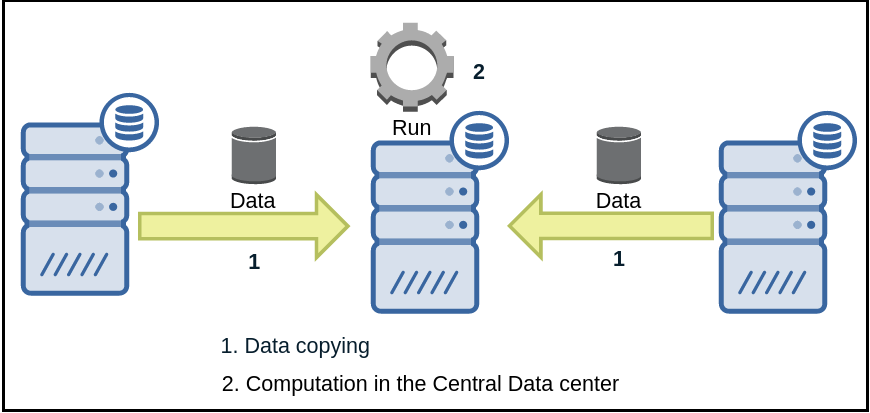
\includegraphics[width=3.2in]{1.png}
\caption{Centralized Approach}
\label{centralized}
\end{figure}
\end{center}

This centralized approach is predominant in most practical settings. 
There are mainly two reasons behind its popularity. 
\begin{enumerate}
\item There are lots of frameworks that have already been established for centralized learning approach. That is why centralizing the data is the easiest way to reuse existing data analysis frameworks \cite{1,2,3}
\item Learning algorithms are highly communication intensive. Thus it is assumed that they will note be properly responsive to cross data center execution.
\end{enumerate}
For these reasons, this centralized approach is consistent with reports on the infrastructures of other large organizations, such as Facebook \cite{4}, Twitter \cite{5}, and LinkedIn \cite{6}. 

However the centralized approach has two shortcomings.
\begin{enumerate}
\item While making multiple copy of data at the central data center, it consumes a good amounts of inter data center bandwidth. Since inter data center bandwidth is expensive, it is not easy to increase it according to the necessity \cite{7,8,9,10}.
\item While creating copy of data, it may be a case that data is crossing national borders. However, in current workd data sovereignty is a growing concern that might create a big limitation in this aspect \cite{11,12}.

\end{enumerate}

\subsection{Distributed Approach}
In the distributed approach, raw data is kept in their corresponding data centers. Every data center does a portion of the execution that is only on the data of that data center. The final analysis takes pales by passing small amount of information among the data centers. 
\begin{center}
\begin{figure}[!htbp]
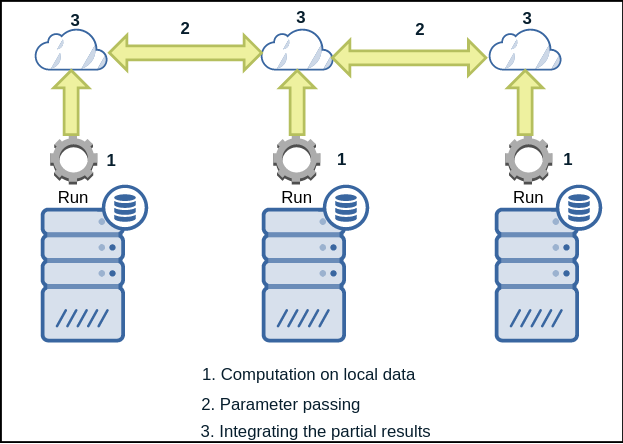
\includegraphics[width=3.2in]{2.png}
\caption{Distributed Approach}
\label{distributed}
\end{figure}
\end{center}

So according to Figure \ref{distributed}, we can see this approach includes three steps:

\begin{enumerate}
\item \textbf{Local Computation} Whenever the command of starting of any learning process is issued every data center start a partial computation on its own data. They create necessary high level information on data that will be needed in the final computation.

\item \textbf{Parameter Passing} Data centers communicate among themselves and share valuable information.

\item \textbf{Final Computation} By integrating the partial results data centers make the final computational model.
\end{enumerate}

In this way distributed solutions can achieve much lower cross data centers bandwidth utilization, and thus substantially lower cost for large-scale analysis tasks. As the current world has got a concern about `Big Data' and `Data Sovereignty', the distributed approach seems to be more efficient. 

\section{PCA as Data Analytic Approach}
Principal component analysis (PCA) is a statistical procedure that uses an orthogonal transformation to convert a set of observations of possibly correlated variables into a set of values of linearly uncorrelated variables called principal components \cite{13}. The number of principal components is less than or equal to the smaller of the number of original variables or the number of observations. This transformation is defined in such a way that the first principal component has the largest possible variance and each succeeding component in turn has the highest variance possible under the constraint that it is orthogonal to the preceding components. As we can use PCA for dimensionality reduction, it can be used as a preprocessing step  in many machine learning algorithms that do not perform well with high-dimensional data. Therefore we can easily realize that PCA is an excellent tool for big data analysis. 

There are several ways to perform PCA. Eigen Value Decomposition (EVD) of covariance matrix and Singular Value Decomposition (SVD) are two basic and most common ways \cite{14}. These methods usually perform better on small datasets on a single machine. But in distributed settings and for big data, they introduce a new set of difficulties; they do not scale well to high dimensional data and are inefficient in terms of computation and communication cost \cite{elgamal}. To overcome these difficulties, two other methods, Stochastic SVD (SSVD) \cite{16} and Probabilistic PCA (PPCA) \cite{17} are used in practice. But unlike the other methods to calculate principal component (i.e. EVD of covariance matrix, SVD, SSVD), PPCA has two important advantages. It has the ability of handling missing data and calculating probabilistic model to generate synthesized data \cite{18}. These features are best suited for big data as missing values are prevalent in this case and a probabilistic model of the data will be more effective for analytical purposes.

Despite of being an excellent tool of data analysis, we lack in proper approach of PPCA in big data analysis. We saw a decent approach of making scalable PCA or \textit{sPCA} in a distributed environment  \cite{elgamal}.  It was designed for data analysis on large datasets on distributed commodity clusters. But unfortunately this approach is not capable of handling datasets with very large dimension, we can say data that is at the same time tall and wide. Moreover data sovereignty is not ensured. There was no method of performing PCA on big data located at different geographic location which involves independent computation at different clusters and accumulation of intermediate results. 

In this paper, we explore these two issues in depth. We will propose a solution which is capable of handling \textit{Tall and Wide} big data and at the same time can perform on geographically distributed datasets where there is no provision of passing raw data across the data center. 


The rest of this paper is organized as follows. In Section II, we discuss the background of PPCA showing its valuable advantages as well as some limitations. In Section III, we analyze already established approach \textit{sPCA}. We present our proposed implementation of PPCA on geographically distributed \textit{Tall and Wide} big data in Section IV. We justify our contribution in Section V. Section VI presents some of the properties of our approach and Section VII presents our experimental evaluation. Finally, Section VIII concludes the paper.



\section{Our Focus}
In current world, the rate of generation of data is quite large. We live in an age of Big Data and Internet of Things (loT). The term Big Data is not really an overstatement. Numerous web services share and collect data of huge scale, typically in terabytes range, and the data includes various aspects of users, for example, clicks, visits, likes, shares, comments, reviews, ratings, tweets, photos, videos etc. Apart from these web services, big data is also generated by countless sensors all around the globe to gather valuable information about respective fields. For example, closed circuit cameras recording is a good source of big data. In a nutshell, every electronic device, Internet services, embedded system and sensor the globe produce and transmit data and big data is being generated by these multiple sources at an alarming velocity, volume and variety.

For researchers, however, big data brings new sets of challenges like how to efficiently and
effectively handle big data in commodity computers, how to apply conventional algorithms, how
to properly manage big data in distributed setting etc. Specially, in field of machine leaning and
Pattern recognition, big data poses a threat, because the conventional algorithms were designed
solely to fulfill its purpose where entire dataset can fit in memory. Distributed setting was not
taken into consideration. In nutshell, to extract any meaningful insight from this big data, we
need powerful tools to analyze it, elastic frameworks to cope up with its sheer volume and most
importantly we have to rethink and redesign existing algorithms which are most suitable for
smaller sized data-set and do not take advantage of clusters.

In this chapter we will discuss the present issues that we are going to take into consideration in our research. We will indicate the challenges we targeted and in later chapters we will give our proposals in order to minimize these challenges in data analysis.

\subsection{Tall and Wide Data}
In general, the width of data means the number of features that each data sample is comprised of. In present world, this features count is increasing at large scale. The feature count or width of data sample can also be named as ``Dimension of Data". One of the most effective use of PCA is dimensionality reduction. Many machine learning algorithms are not capable of handling data with large dimension. Therefore, we can use PCA to reduce the width of data then fit them in some kind of machine learning model. This present some kind of new challenge. The present PCA algorithms are not that much capable of handle very wide data that is tall also. Therefore before making the data suitable for machine learning models by dimensionality reduction, the PPCA algorithm has to deal with the curse of tall and wide data. The present implementation of \textit{sPCA} done good number of optimization to make efficient use of memory. Still it is not capable of handling tall and wide data. The memory overflow occurs while computing the intermediate results. 
\subsection{The Blessings and Curses of Geo Distributed Data}
The data generation at different geographic location has made the data geographically distributed. Data is being generated mainly at the location close to the end user. There are several advantages of such geographically distributed data such as (1) Assurance of faster data access to the end user (2) Protection of national privacy and data sovereignty (3) Sparsity of data center of the same company (4) Advanced development in business sector. 

Despite of having some advantages, geographical distribution of data posses some kind of challenges in data analytic. It creates a scenario where there will be no global view of data during any kind of data analysis. This demands a new technology in data the field of data analysis. Moreover in case of breakdown of any particular data center, the data analysis technique has to be able to handle missing data. Data clusters located at different location might not have the same kind of configuration i.e. the clusters might be heterogeneous. 

Taking these challenges, the data analysis algorithm needs to be capable of performing partial analysis on the tall and wide data at every individual data clusters and creates some kind of intermediate results and then needs to accumulate them in an time efficient approach to produce the final results.




\section{Background}
We will discuss some background of PPCA according to \cite{bishop}. We can obtain a probabilistic formulation of PCA by introducing a Gaussian latent i.e. unobserved variable mode. This kind of model is highly related to statistical factor analysis. A latent variable model seeks to relate a $D$-dimensional observation vector $\pmb{y}$ to a corresponding $d$-dimensional vector of latent variables $\pmb{x}$ where the relationship is linear:
\begin{equation}
\pmb{y} = \pmb{Wx}+ \pmb{\mu} + \pmb{\epsilon}
\label{PPCA:eq1}
\end{equation}
Where:
\begin{itemize}
\item $\pmb{y}$ is a $D$ dimensional observed data vector
\item $\pmb{x}$ is a $d$ dimensional latent variable
\item $\pmb{W}$ is a $D \times d$ transformation matrix
\item the columns of $\pmb{W}$ are the principal components
\item $\pmb{\mu}$ is the dimension wise mean vector of $\pmb{y}$. This parameter allows the data to have non zero mean
\item $\pmb{\epsilon}$ is a $D$-dimensional zero-mean  noise variable
\item Here $\pmb{x}$, $\pmb{\epsilon}$, $\pmb{y}$ are normal distributed i.e. Gaussian distributed
\begin{align*}
\pmb{x} &\sim \mathcal{N}(\pmb{0},\pmb{I})\\
\pmb{\epsilon} &\sim \mathcal{N}(\pmb{0},\pmb{\sigma^2I})\\
\pmb{y} &\sim \mathcal{N}(\pmb{\mu},\pmb{WW}^T+\pmb{\sigma^2})
\end{align*}
where $\pmb{x} \sim \mathcal{N}(\pmb{u},\sum)$ denotes the Normal distribution with $\pmb{u}$ mean and $\sum$ covariance matrix.
\end{itemize}

The motivation is that, with $d < D $, the latent variables will offer a more parsimonious explanation of the dependencies between the observations. The model parameters may thus be determined by maximum-likelihood, As there is no closed-form analytic solution for finding $\pmb{W}$ and $\pmb{\sigma}^2$, their values must be obtained via an iterative procedure.

The use of the isotropic Gaussian noise model $\mathcal{N}(\pmb{0},\pmb{\sigma^2I})$ for   in conjunction with equation (\ref{PPCA:eq1}) implies that the $\pmb{x}$-conditional probability distribution over $\pmb{y}$-space is given by:
\begin{equation}
\label{PPCA:eq2}
\pmb{y|x} \sim \mathcal{N}(\pmb{Wx}+\pmb{\mu}, \pmb{\sigma}^2\pmb{I})
\end{equation}
With the marginal distribution over the latent variables also Gaussian and conventionally defined by $\pmb{x} \sim \mathcal{N}(\pmb{0},\pmb{I})$, the marginal distribution for the observed data $\pmb{y}$ is readily obtained by integrating out the latent variables and is likewise Gaussian:
\begin{equation}
\label{PPCA:eq3}
\pmb{y} \sim \mathcal{N}(\pmb{\mu},\pmb{C})
\end{equation}
where the observation covariance model is specified by $\pmb{C}=\pmb{WW}^T+\pmb{\sigma^2}$. given $N$ observations $\{\pmb{y_n}\}^N_1$ as the input data, the log likelihood of data is given by:
\begin{align}
\label{PPCA:eq4}
{\mathcal{L}(\{ \pmb{y_r}\}^N_1)} &= \sum_{n=1}^N \ln{p(\pmb{n_r})} \nonumber \\
&= -\dfrac{1}{N}\{D*\ln(2\pi) + \ln|\pmb{C}| + tr(\pmb{C}^{-1}*\pmb{S})\}
\end{align}
where $\pmb{S}$ is the sample covariance matrix of data $\pmb{\{y_r\}}$ given by $
\pmb{S} = \dfrac{1}{N} \sum_{n=1}^N (\pmb{y_r - \mu})(\pmb{y_r - \mu})^T$ and $tr(\pmb{M})$ is the trace of matrix $\pmb{M}$

According to \cite{bishop}, the likelihood of $\pmb{W}$ and $\pmb{\sigma}$ is maximized when:
\begin{equation}
\label{PPCA:eq7}
\pmb{W}_{ML} = \pmb{U}_d \sqrt{\pmb{\Lambda}_d - \sigma^2\pmb{I}}\pmb{R}
\end{equation}
It may also be shown that for $\pmb{W} = \pmb{W}_{ML}$, the maximum-likelihood estimator for $\sigma^2$ is given by:
\begin{equation}
\label{PPCA:eq8}
\sigma^2_{ML} = \dfrac{1}{D - d} \sum_{i=d+1}^D \lambda_i
\end{equation}

\subsection{An EM Algorithm for Probabilistic PCA}
In the EM approach to maximising the likelihood for PPCA, we consider the latent variables  $\{\pmb{x}_n\}$ to be `missing' data and the `complete' data to comprise the observations together with these latent variables. The corresponding complete-data log-likelihood is then:

\begin{equation}
\label{PPCA:eq22}
\mathcal{L}_C = \sum^N_{n=1} \ln {p(\pmb{y}_n),\pmb{x}_n)} 
\end{equation}

In order to make the EM algorithm look simple we define:
\begin{align*}
\pmb{E}_n &= \langle \pmb{x}_n \rangle\\
\pmb{F}_n &= \langle \pmb{x}_n\pmb{x}_n^T \rangle\\
\pmb{Y}_m &= (\pmb{y}_n - \pmb{\mu})\\
{Frob(\pmb{Y}_m)} &= || \pmb{y}_n - \pmb{\mu} ||^2
\end{align*}
Therefore, we can write the EM steps with simplified notations:
\begin{align}
\label{PPCA:EM}
\text{\textbf{E-step:}} \ \ \ \ \  \pmb{E} &= (\pmb{Y}_{m})\pmb{W}\pmb{M}^{-1} \\
\label{PPCA:EM1}
\text{\textbf{E-step:}} \ \ \ \ \  \pmb{F} &= \pmb{E}^T\pmb{E} + \mathlarger{\sigma}^2\pmb{M}^{-1}\\
\label{PPCA:EM2}
\text{\textbf{M-step:}} \ \ \ \ \pmb{\widetilde{W}} &= (\pmb{Y}_m^T\pmb{E})\pmb{F}^{-1} \\
\label{PPCA:EM3}
\text{\textbf{M-step: }}\ \ \ \mathlarger{\sigma}^2 &= \dfrac{1}{ND} \left[    Frob(\pmb{Y}_m) - 2 \mathlarger{\sum}^N_{n=1} \pmb{E}_n^T \widetilde{\pmb{W}}{\pmb{Y}_m}_n \right.\\& \left.+ tr \left(\pmb{F} \widetilde{\pmb{W}}^T\widetilde{\pmb{W}}  \right) \right] \nonumber
\end{align}

Iterating Equation (\ref{PPCA:EM}), (\ref{PPCA:EM1}), (\ref{PPCA:EM2}), (\ref{PPCA:EM3}) upto convergence, we can make a good approximation of both $\pmb{W}$ and $\pmb{\mathlarger{\sigma}^2}$.
The basic algorithm of PPCA is given below:

\begin{algorithm}[!htbp]
\label{basic}
\caption{Basic PPCA}
\begin{algorithmic}[1]
\State $W = normrnd(D,d)$
\State $ss=normrnd(1,1)$
\State $Y_m=columnMean(Y)$
\State  $Y_c=Y-Ym$
\While {$(!Stop\_Condition)$}
	\State $M = W^T * W + ss * I$
	\State $X = Y_c * W * M^{?1}$
	\State $XtX = X^T * X + ss * M^{-1}$
	\State $YtX = Y_c^T * X$
	\State $W = YtX \times$ \textit{invert($XtX$)}
	\State $ss2 = trace(XtX * W^T * W)$
	\State $ss3= \sum_{n=1}^N X_n * W^T * {Y_c}_n$
	\State $ss = (||Y c||^2_F + ss2-2 * ss3)\times N^{-1} \times D^{-1}$
\EndWhile
\end{algorithmic}
\end{algorithm}


\section{Recent Implementation of \textit{sPCA}}
\cite{elgamal} presented a  scalable implementation of Probabilistic PCA for distributed platforms such as MapReduce and Spark. 
\subsection{Special Features}
The implementation of \textit{sPCA} has a good number of features:
\subsubsection{Mean Propagation to Leverage Sparsity}
The first optimization we propose is the mean propagation idea, which preserves and utilizes the sparsity of the input matrix $\pmb{Y}$. PPCA requires the input matrix to be mean-centered, meaning that the mean vector $\pmb{\mu}$ must be subtracted from each row of the original matrix $\pmb{Y}$. Large matrices, however, are mostly sparse, with many zero elements. Sparse matrices can achieve a small disk and memory footprint by storing only non-zero elements, and performing operations only over non-zero elements. Subtracting the non-zero mean from the matrix would make many elements non-zero, so the advantage of sparsity is lost.

To avoid the problems of subtracting the mean, they keep the original matrix $\pmb{Y}$ and the mean $\pmb{\mu}$ in two separate data structures. they did not subtract the mean $\pmb{\mu}$ from $\pmb{Y}$. Rather, they propagate the mean throughout the different matrix operations.
\subsubsection{Minimizing Intermediate Data}
Intermediate data can slow down the distributed execution of any PCA algorithm, because it needs to be transferred to other nodes for processing to continue. Their second optimization is job consolidation, which means merging multiple distributed jobs into one in order to reduce the communication between these jobs.
\subsubsection{Efficient Matrix Multiplication}
PPCA requires many matrix multiplications, which are expensive operations in a distributed setting. To appreciate the techniques that \textit{sPCA} employs to overcome the inefficiency of matrix multiplication, they briefly explain different possible implementations of this operation.
\subsubsection{Efficient Frobenius Norm Computation}
The PPCA algorithm requires computing the Frobenius norm of the mean-centered input matrix. To solve this problem, they design an algorithm which does not even require creating the dense vector. Many machine learning algorithms compute various norms of matrices. The proposed method for optimizing the computation of the Frobenius norm can be extended to other matrix norms using similar ideas. Thus, this simple optimization can benefit several other machine learning algorithms.
\subsection{Limitations}
Despite of having some wonderful features \textit{sPCA} has some limitations also. We can discuss these limitations from two aspects.

\begin{enumerate}
\item The approach is not applicable for high dimensional data or we can say tall and wide big data. Though the approach has done some efficient use of memory by reducing the generation of intermediate data, it still runs out of memory while running on big data whose vertical dimension is in the range of millions. We failed to run \textit{sPCA} on dataset of dimension $10M\times5M$ in our set-up cluster where we have machines with $64GB$ of RAM.\\   

\item There was no implementation on geographically distributed big data. In current world where data is distributed across national border to ensure fast access and national data sovereignty, it is necessary to be capable of doing data analysis on such geo-distributed data. However, \textit{sPCA} did not indicate a process of generating some kind of partial result and later accumulate them to produce the final analytic results.
\end{enumerate}

\section{Our Proposed Approach}
As discussed before, we are interested in presenting an approach that will resolve the memory limitation problem and hence give an systematic way to run \emph{PPCA} on geographically distributed data. 

\subsection{Handling Tall and Wide Big Data}
Our first concern was to make commodity computers capable of performing PPCA on such big data which has very large sample count as well as very high dimension i.e. very large feature count. In this respect we will follow the approach from \cite{elgamal} with some necessary improvements. To have a distributed settings we will take advantage of cluster computing. In case of very wide data the size of principal subspace $W$ is going to be very big. Therefore, we have to treat the principal subspace $W$ as big data also. Performing PPCA in the conventional approach on tall and wide big data will result in the overflow of memory. Therefore, we have to make some kind of improvements to make the approach capable of handling tall and wide big data in case of performing PPCA overcoming the memory scarcity. The steps of performing PPCA in a single cluster is as follows:

\subsubsection{\textbf{Step 1 - Partition of Principal Subspace $W$}}\hspace*{\fill} \\
For data with the dimension $N \times D$ we will get a principal subspace of dimension $D \times d$ where $d$ denotes the number of principal components we want. Working with full horizontal $D$ dimension of $W$ will result in memory overflow. Therefore, we will make $n$ horizontal partition of $W$ and create $W_1, W_2, \dots , W_n$. As a result each stage of creating $W$ will consists of $n$ smaller stages of creating $W_i$. 


\subsubsection{\textbf{Step 2 - Data Partition}}\hspace*{\fill} \\
As we are partitioning the horizontal $D$ dimension of principal subspace $W$, we are indirectly make vertical partition of our data of $N \times D$. At each iteration of generating $W$, we have to work on a specific horizontal segment of it. Therefore, we have to work with only that segment of dimension of our data. In that sense we can say that we are creating vertical partition of our main data matrix. It might be a case that data is pretty large that even a distributed setting with multiple machines might not be capable of performing the PPCA task by keeping the full data in memory. In such case our approach can be memory efficient by loading only a single segment of data at each iteration. This will help in memory intense tasks.  

\subsubsection{\textbf{Step 3 - Expectation Step and Omission of Noise Model}}\hspace*{\fill} \\
From Algoritm \ref{basic} we can see that computation of $\pmb{\sigma ^2}$ involves $X$ which is going to a $N \times d$ matrix. Therefore, passing such big data will result in communication bottleneck. For simplicity of computation and minimizing the inter data cluster communication, we will omit the noise calculation. 

On the other hand, in order to take advantage from segmented computation, we have to make some changes in the Expectation and Maximization steps of the main \textbf{EM Algorithm} of PPCA. 
Omitting the noise model and from Equation (\ref{PPCA:EM}), (\ref{PPCA:EM1}) and Algorithm \ref{basic}, the E-Steps are:

\begin{align}
\label{1}
M &= W^T * W\\
\label{2}
X &= Y_c * W * M^{-1}\\
\label{3}
XtX &= X^T * X\\
\label{4}
YtX &= Y_c^T * X
\end{align}

In our approach $M$ is not going to be produces at the start of the process as ot depends on $W$ which will be segmented in our system. Therefore we are going to produce multiple number of $M$'s and accumulate them to produce the final $M$. The steps equivalent to Equation \ref{1}: 
\begin{align}
\label{5}
M_i &= W_i^T * W_i \\
\label{6}
M &= \sum^n_{i = 1} M_i
\end{align}
Similar thing will happen for producing $X$ of Equation \ref{2}:
\begin{align}
\label{7}
X_i &= {Y_c}_i * W_i\\
\label{8}
X &= \sum^n_{i = 1} X_i
\end{align}
%We can see that as soon as $M_i$'s and $X-i$'s are generated at the end of $n$ segmented iterations according to Equations \ref{5} and \ref{7}, we can generate $M$ and $X$ by using Equations \ref{6} and \ref{8}. Then Equation \ref{9} will be executed to produce final $X$
Steps to produce $XtX$:
\begin{align*}
    X   &= X * M^{-1}\\
    XtX &= X^T * X\\
        &= (X * M^{-1})^T*(X * M^{-1})\\
        &= {M^{-1}}^T*X^T*X*M^{-1}\\
        &= {(M^{-1})}^T*(X^T*X)*(M^{-1})
\end{align*}
Similarly we will produce $YtX$
\begin{align*}
    X   &= X * M^{-1}\\
    (YtX)_i &= {Y_c}_i^T * X\\
        &= ({Y_c}_i^T * X) * M^{-1} 
\end{align*}

\subsubsection{\textbf{Step 4 - Maximization Step}}\hspace*{\fill} \\
As we have mentioned earlier we are omitting the calculation of variance $\pmb{\sigma ^2}$. Therefore, our maximization step gets limited to the only computation of new $W$. As we are generating $W$ in a segmented approach, at iteration $i$ we are going to generate $W_i$ as follows:
\begin{equation*}
    Wi = (YtX)_i * XtX^{-1}
\end{equation*}
Here $(YtX)_i$ is the $YtX$ generated from $Y$ for the range of dimension corresponding to $i$.






where data is partitioned vertically in different machines of the same cluster. 

















\begin{figure}[!htbp]
\label{flow}
\centering
\frame{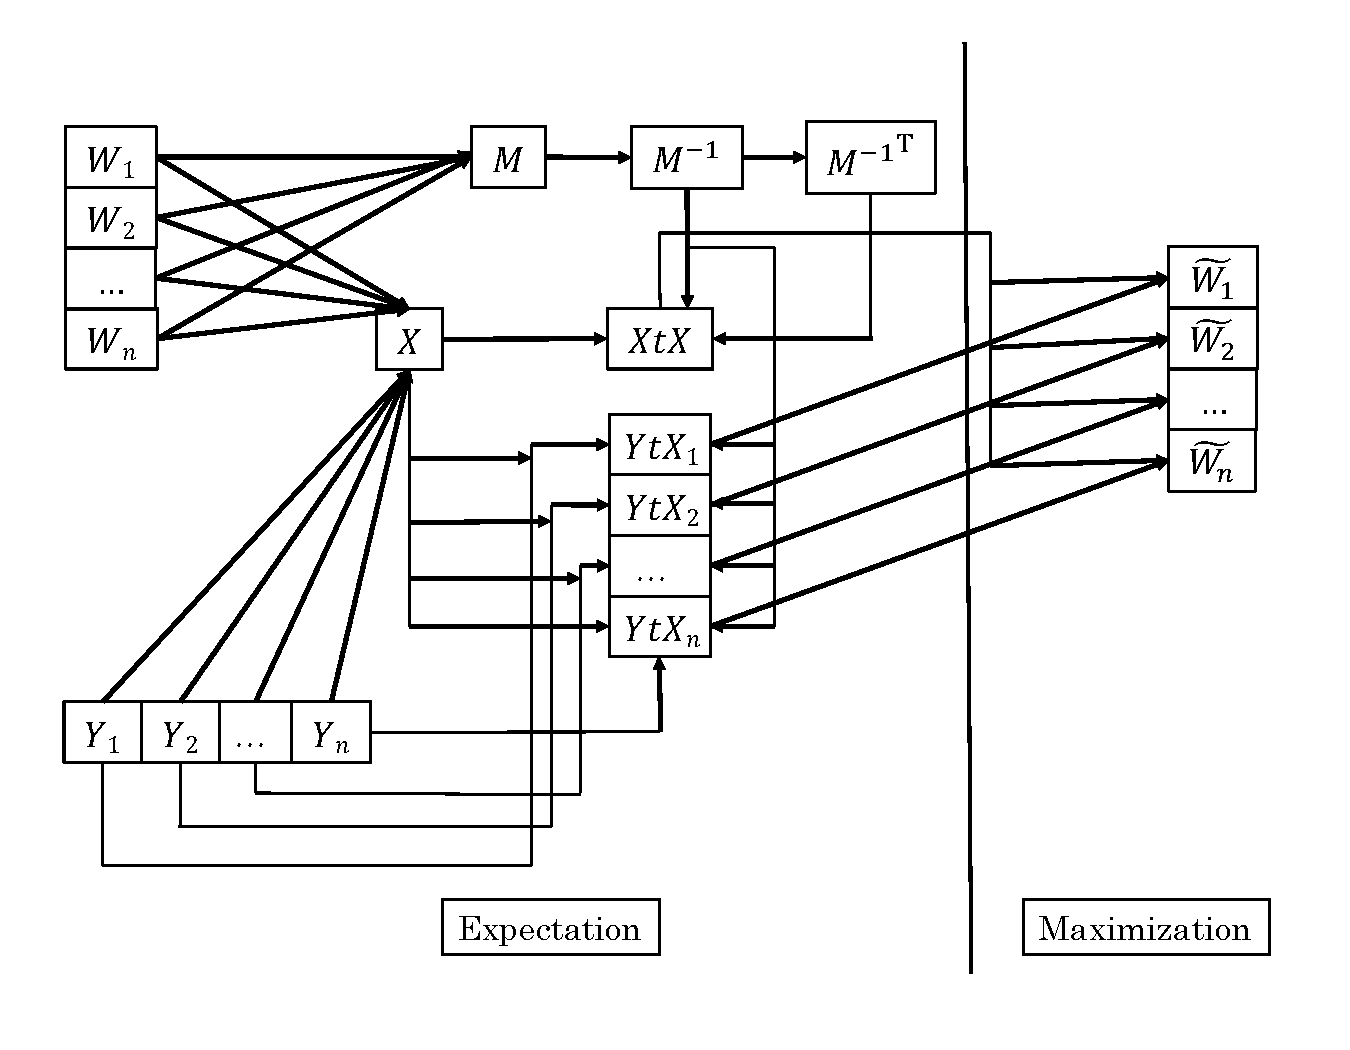
\includegraphics[width=3.5in]{flow.pdf}}
\caption{Flow Graph of Algorithm \ref{tallnwide}}
\end{figure}

\subsection{Accumulation of partial results from geographically distributed clusters}
As we mentioned earlier our data will be geographically distributed. That means we are not going to have any global view of data and no raw data passing is allowed to preserve national data sovereignty. Therefore, the partially computed results have to accumulated to produce the final result. We had the intention to minimize (a) the volume of data to be transmitted throughout the whole process and (b) accumulate the partial results in a way that will ensure the minimum accumulation time.
The former was handled in the previous subsection. In The later part we are going to be use some graph theory properties to achieve what we desire.

At each iteration of PPCA we are generating a segment of our principal subspace $W$. An arbitrary segment can can be denoted as $W_i$. Whenever one such segment is newly generated, each data cluster will call the \textbf{Accumulation} procedure from Algorithm \ref{accum}. The full accumulation process that we are proposing can be presented as follows:

\subsubsection{\textbf{Step 1: Generating The Initial Graph}}\hspace*{\fill} \\
The data clusters that are geographically distributed are connected by high or low bandwidth connection based on their location. According to \cite{nokia} and \cite{fujitsu}:
\begin{itemize}
\item Clusters that are located at the same region  generally have connection of bandwidth in the range above $100gbps$ 
\item Clusters that are located at nearby regions  generally have connection of bandwidth in the range of $10$-$100gbps$ 
\item Clusters that are located at different and distanced regions  generally have connection of bandwidth in the range of $1$-$10gbps$ 
\end{itemize}
At the start of the full PPCA process, every data cluster will check the bandwidth of the  connections of every other clusters it is connected with and generate a graph. The full process will results in a complete graph if there is an interconnection between every two data clusters. In this graph every node $v_i$ will represent a data cluster $DC_i$ while edge $e_{ij}(cost)$ between nodes  $v_i$ and  $v_j$ denotes that   $DC_i$ and $DC_j$ are connected at a b/w using which certain amount of data needs $cost$ amount of time to transmit among the two vertices. The Figure \ref{G} shows such a generated graph with $10$ data clusters.


\begin{figure}[!htbp]
\label{G}
\centering
\frame{\includegraphics[height=2.1in,width=2.8in, page=3]{t.pdf}}
\caption{Generated Graph $G$ According to Step-1}
\end{figure}

\subsubsection{\textbf{Step 2: Generating MST}}\hspace*{\fill} \\
Using the graph generated in \textit{step 1}, every node will generate a \textit{Minimum Spanning Tree} to make a connected component with the least cost using time required to transmit data as the cost of the tree edges. 
Figure \ref{MST} shows the MST generated from graph from Figure \ref{G}.

\begin{figure}[!htbp]
\label{MST}
\centering
\frame{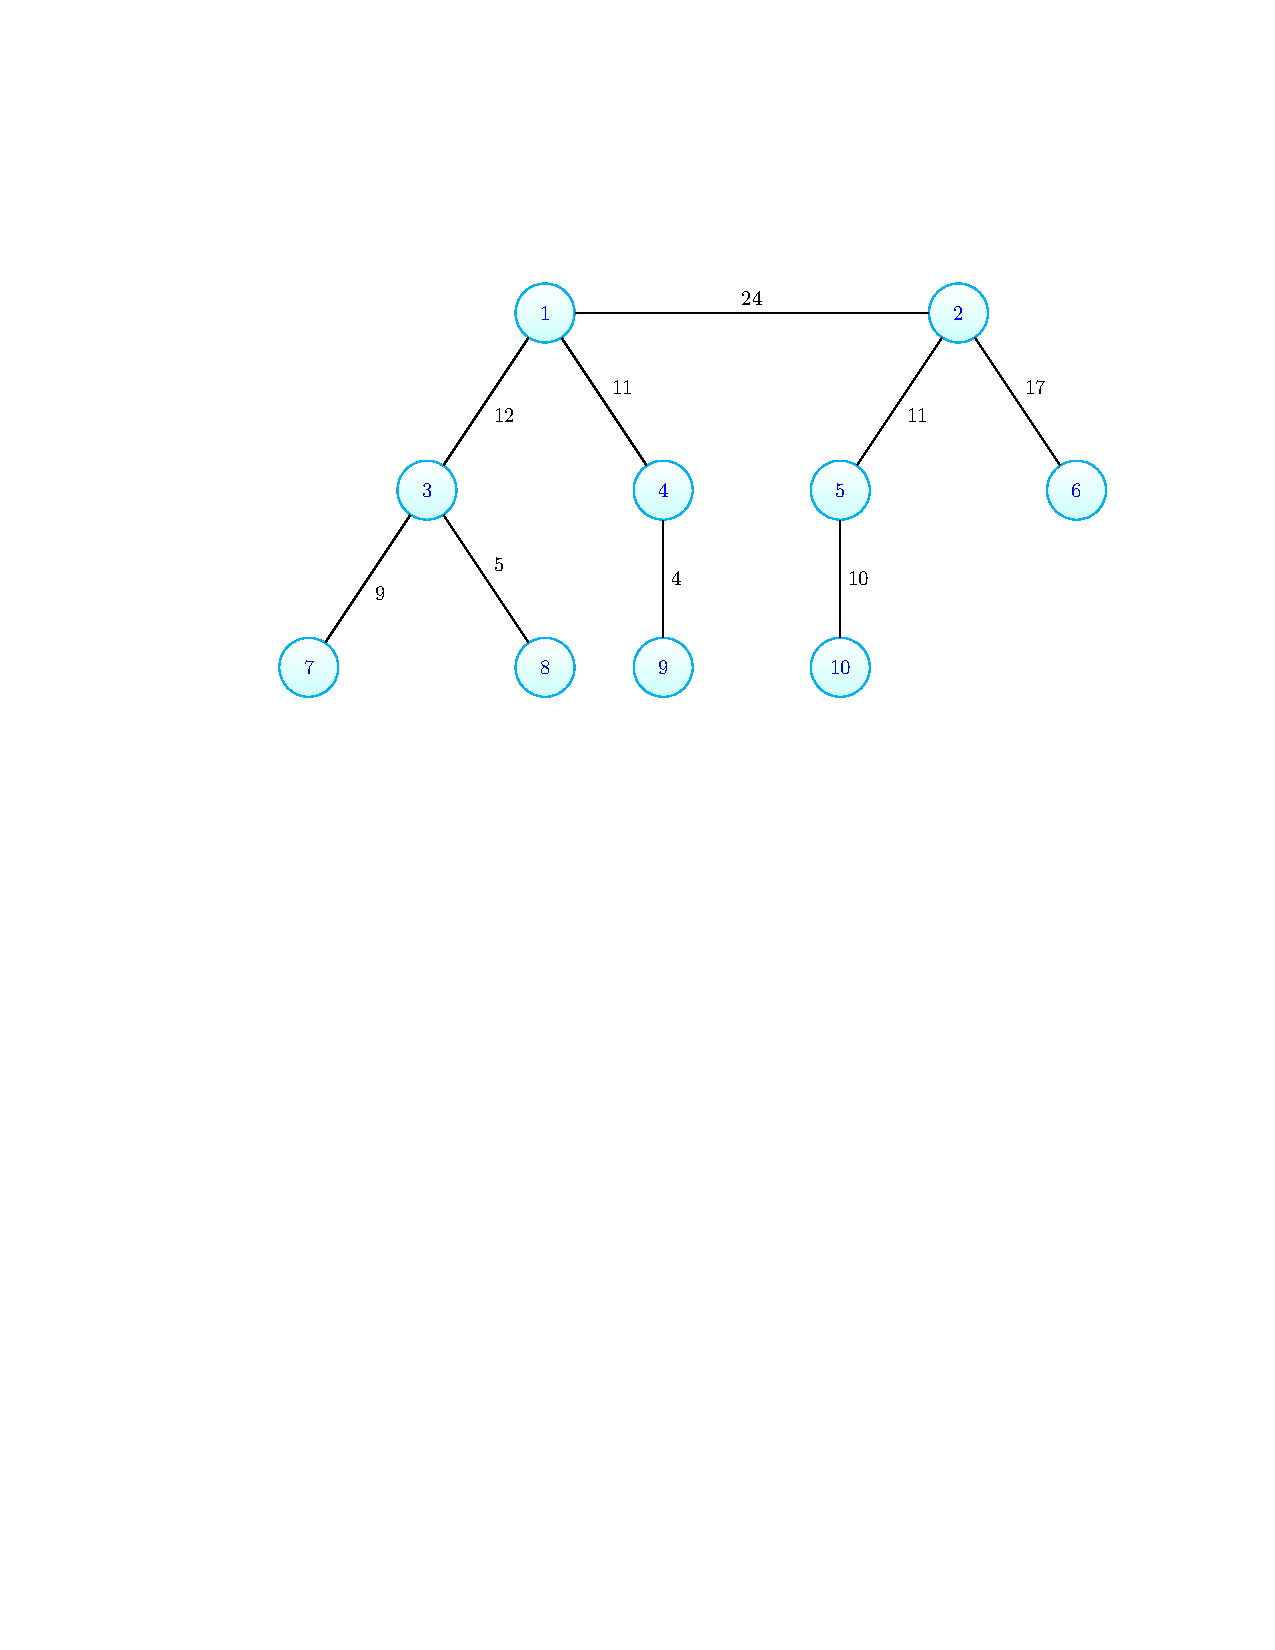
\includegraphics[width=2.8in, page=1]{t.pdf}}
\caption{Generated MST According to Step-1 from Graph $G$}
\end{figure}


\subsubsection{\textbf{Step 3: Sub Tree Generation for Parallel Accumulation}}\hspace*{\fill} \\
We are going to generate two sub trees from the MST generated in \textit{Step 2} according to Algorithm \ref{algo6}. We will intended to choose the maximum time consuming edge $e_m$ and make a sub tree rooted at each of the end vertices of that edge. This will be done to make the process to use the maximum time consuming link only once while accumulating data. What we are trying to achieve is that all the data cluster nodes at each of the sub trees now can perform the accumulation task in parallel. Accumulation will be done in  bottom up direction. 
Therefore two accumulated results will  available at the two root data nodes. At that point a single exchange will results in having the final result at each of the root node of the two sub trees.

From this sub tree generation with using the node information, every data node will learn the information of its child nodes and parent nodes. During accumulation it will accumulate results from its child data nodes and notify the completion of it accumulation to its parent node.  

What we keep in mind that this  subtree formulation method might create some kind of unbalanced subtree. Figure \ref{uMST} shows such an unbalanced sub tree where $subtree1$ has a total cost of $51$ and $subtree1$ has a total cost of $21$.



\begin{figure}[!htbp]
\label{uMST}
\centering
\frame{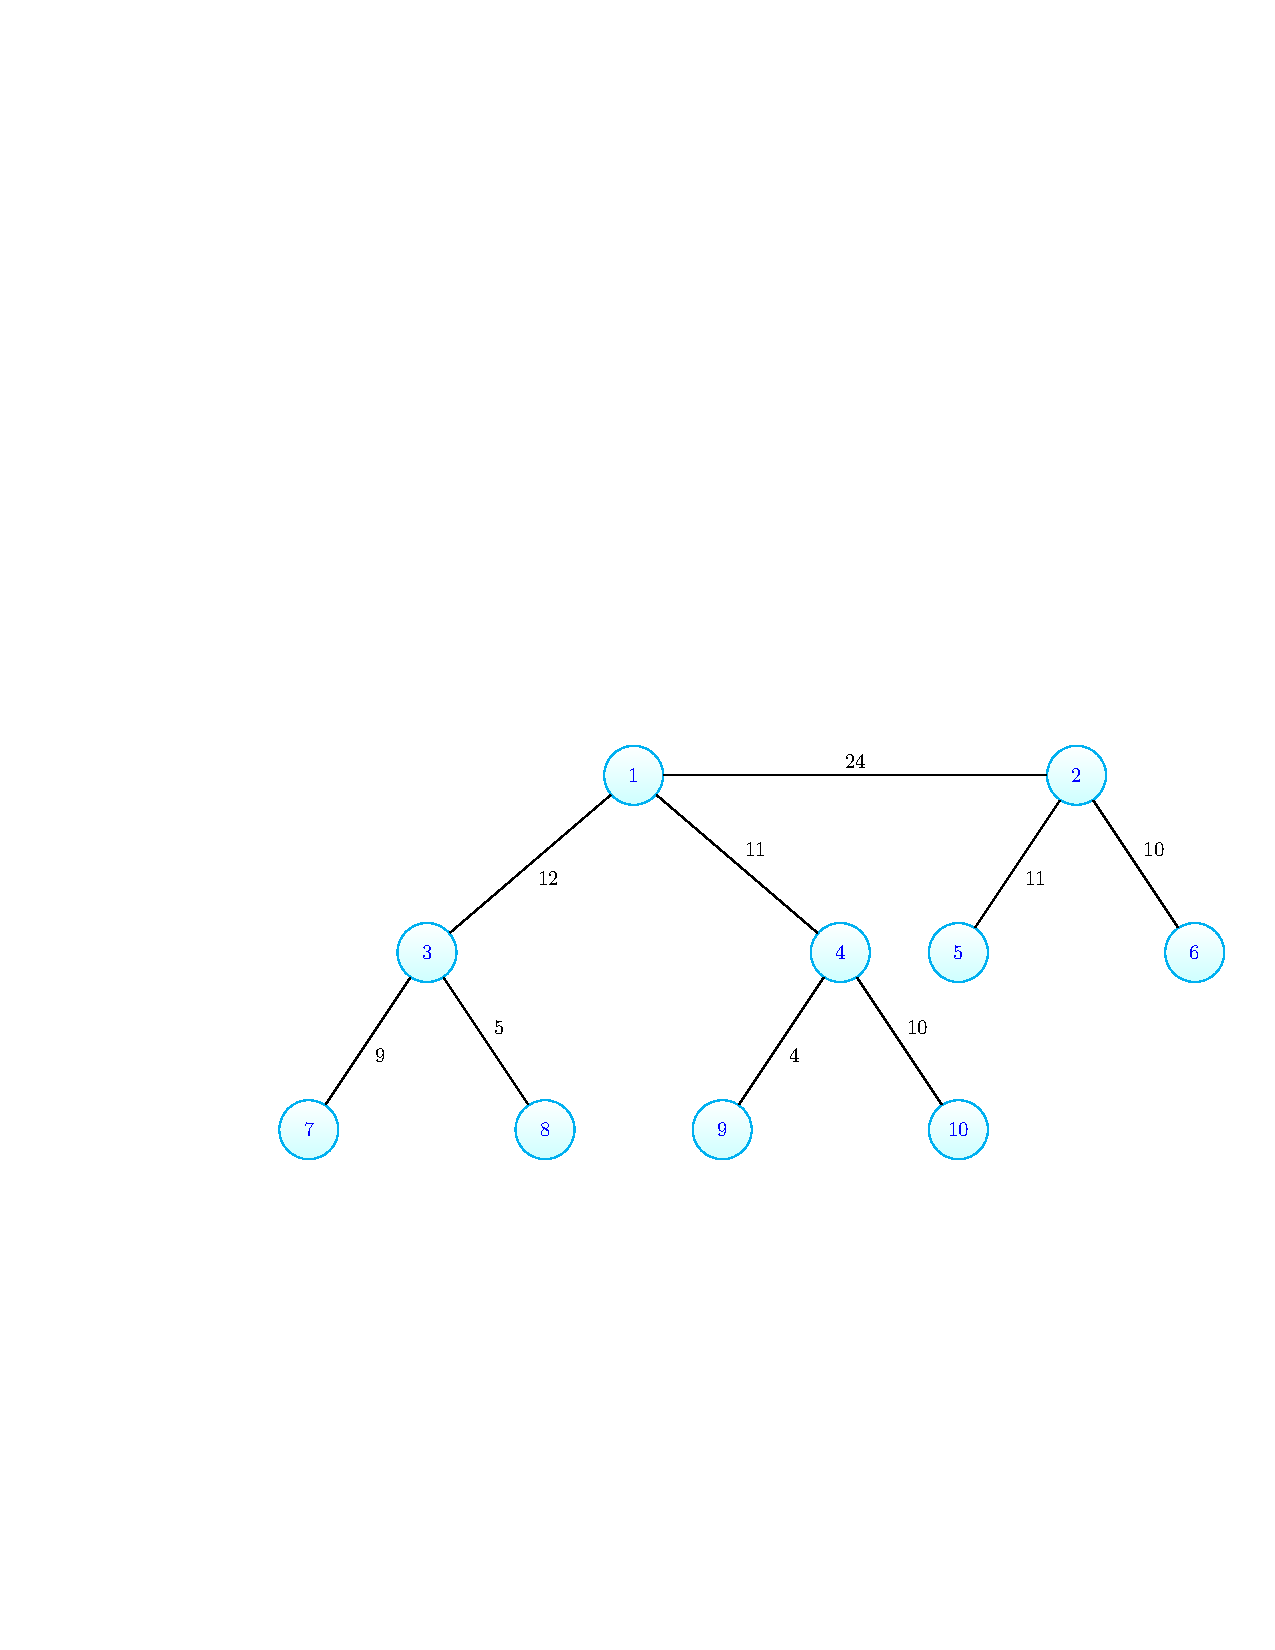
\includegraphics[width=2.8in, page=1]{t1.pdf}}
\caption{Unbalanced Sub Tree}
\end{figure}

To overcome such condition, we will then make a trade off between choosing the highest time consuming link and the balanced cost of the sub trees. To make the sub tree costs more or less balanced we will try to take the next maximum time consuming link and so on. 
\subsubsection{\textbf{Step 4: Redistribution of Final Accumulated Result}}\hspace*{\fill} \\
Whenever each of the root nodes completes the accumulation of its own sub tree, it will wait for the other root to complete. After that it will access the partially accumulated result from the other root node and complete the full computation. At this stage it will distribute the final result by pushing it through the links connecting to its neighbours. As there will be dedicated links, the result can be sent to each of the neighbours at the same time. Whenever ant node in a sub tree receives the final result it will also redistribute it to its child nodes in the tree configuration. The job will end with the leaf data nodes receiving the final accumulated result.





\newcommand\tab[1][.5cm]{\hspace*{#1}}
\begin{algorithm} [!htbp]
	\label{tallnwide}
  \caption{PPCA on Tall and Wide Big Data}
  \begin{algorithmic}[1]
  \State \textbf{createMyInfo()}
  \State $myInfo$ = \textit{readFile}($myInfo$)
  \State Let $Range[1.....partitionCount+1]$ be an array %containing range value of $W$ 
  \For {i from $1$ to $partitionCount$}
  	\State $Range[i] = (i-1)\times D \div partitionCount$
  \EndFor
  \For {i from $1$ to $partitionCount$}
  		\State $start$ = $Range[i]$  
		\State $end$ = $Range[i+1]$ 
		\State $W_i = $\textit{GenerateRandomW($start, end, d$)}
		\State \textit{saveWInStorage($W_i$)}
  \EndFor
  \State $Stop\_Condition$ = $False$
  \While{($!(Stop\_Condition)$)}
  	  \State $M = null$ 
  \State $X = null$
	\For{i from $1$ to $partitionCount$}
		\State $start$ = $Range[i]$  
		\State $end$ = $Range[i+1]$  
		\State $W_i =$ \textit{loadWFromStorage}($start, end$)
		\State $M_{new} = W_i^T \times W_i$
		\State $M = M$ + $M_{new}$
		\State $X_m = Y_m \times W_i$
		\State \textbf{SegementedXJob($X, Y, X_m, W_i, start, end$)}
	\EndFor
	\State $invM = $\textit{invert($M$)}
	\State $YtX = null$
	\State $XtX = null$
	\For{i from $1$ to $partitionCount$}
		\State $s$ = $Range[i]$  
		\State $e$ = $Range[i+1]$  
		\State \textbf{generateYtXandXtX($YtX,XtX,X,Y,Y_m,i,s,e$)}
		\State $YtX = YtX \times invM$
		\State $XtX = invM^T \times XtX \times invM$
		\State $Wi = YtX \times $ \textit{invert($XtX$)}
		\State \textbf{startAccumulation($myInfo, i$)}
	\EndFor
  \EndWhile
  \end{algorithmic}
\end{algorithm}

\begin{algorithm} [!htbp]
\label{segmented1}
  \caption{SegmentedXJob($X,Y,X_m,W,start,end$)}
  \begin{algorithmic} [1]
	\State $Y_nX$ = $Y$.zip($X$)
	\State $X$ = $Y_nX$.map\{($Y_nX$)$_i \Rightarrow$
	        \State \tab $Y_i$ = ($Y_nX$)$_i$.\textit{arg0()}.\textit{range}($start,end$)
			\State \tab $X_i$ = ($Y_nX$)$_i$.\textit{arg1()}
			\State \tab dotRes = $Y_i \times W$
			\State \tab $X_i$ = $X_i$ + dotRes - $(X_m)_i$
			\State \}
  \end{algorithmic}
\end{algorithm}



\begin{algorithm} [!htbp]
\label{segmented2}
  \caption{SegmentedXJob($YtX,XtX,X,Y,Y_m,i,s,e$)}
  \begin{algorithmic} [1]
	\State $Y_nX$ = $Y$.zip($X$)
	 \If{($i == 1$)}  \Comment{Iteration for First Segment of $W$}
	 		\State $YtXSum = spark.accumultor(newMatrix(D,d))$
			\State $XtXSum = spark.accumultor(newMatrix(D,d))$
	 		\State $Y_nX$.map\{($Y_nX$)$_i \Rightarrow$
	 		\State \tab $Y_i$ = ($Y_nX$)$_i$.\textit{arg0()}.\textit{range}($s,e$)
			\State \tab $X_i$ = ($Y_nX$)$_i$.\textit{arg1()}
			\State \tab $(YtX)_i$ = $Y_i^T \times  X_i$ - $Y_m^T \times X_i$   
			\State \tab $(XtX)_i$ = $X_i^T \times  X_i$
			 \State \tab $YtXSum$.\textit{add($(YtX)_i$)}
			 \State \tab $XtXSum$.\textit{add($(XtX)_i$)}
			\State \}
		\State $YtX = YtXSum$.\textit{value()}
		\State $XtX = XtXSum$.\textit{value()}
	\Else
			\State $YtXSum = spark.accumultor(newMatrix(D,d))$
	 		\State $Y_nX$.map\{($Y_nX$)$_i \Rightarrow$
			\State \tab $Y_i$ = ($Y_nX$)$_i$.\textit{arg0()}.\textit{range}($s,e$)
			\State \tab $X_i$ = ($Y_nX$)$_i$.\textit{arg1()}
			\State \tab $(YtX)_i$ = $Y_i^T \times  X_i$ - $Y_m^T \times X_i$   
			 \State \tab $YtXSum$.\textit{add($(YtX)_i$)}
			\State \}
		\State $YtX = YtXSum$.\textit{value()}
	 \EndIf
  \end{algorithmic}
\end{algorithm}

\begin{algorithm}[!htbp]
	\caption{createMyInfo}
	\begin{algorithmic} [1]
	\State \textbf{Input: }$V: $ Set of Clusters as Vertices
	\State \textbf{Input: }$E: $ Set of Weighted Edges; b/w as Link Weights
	\State \textbf{Input: }$G=\{V,E\}$ Clusters' Distribution Graph
	\State $MST(V_m,E_m)$ = \textit{createMST($G$)}
	\State \{$subTree1, subTree2$\} = \textbf{createSubTree($V_m,E_m$)}
	\State $myInfo$ = \textit{createMyInfo($subTree1, subTree2, myID$)}
	\State \textit{saveMyInfo($myInfo$)}
	\end{algorithmic}
\end{algorithm}

\begin{algorithm} [!htbp]
\label{algo6}
	\caption{createSubTree}
	\begin{algorithmic}[1]
		\State \textbf{Input: }$V_m$, Vertex Set of MST
		\State \textbf{Input:}	$E_m$, Edge Set of MST
		\State \textbf{Output: }$\{subTree1, subTree2\}$, Two Subtrees
		\State sort $E_m$ according to increasing b/w
		\State $done$=$Fasle$
		\While{!$done$}
			\State $e$ = \textit{nextMinimumBWEdge($E_m$)}
			\State $v1$ = $e.startVertex$
			\State $v2$ = $e.endVertex$
			\State $subTree1$ = \textit{subTree($v1$)}
			\State $subTree2$ = \textit{subTree($v2$)}
			\State $cost1$ = \textit{cost($subTree1$)}
			\State $cost2$ = \textit{cost($subTree2$)}
			\If{\textit{(max($cost1,cost2$)}/\textit{min($cost1,cost2$)}$ \leq 1.5$)}
				\State $done = True$
			\EndIf
		\EndWhile	
		\State \textbf{return} $\{subTree1, subTree2\}$
	\end{algorithmic}
\end{algorithm}

\begin{algorithm} [!htbp]
\label{accum}
\caption{startAccumulation}
	\begin{algorithmic}[1]
	\State \textbf{Input:} $myInfo$
	\State \textbf{Input:} $indexOfW$
	\State $W$ = \textit{loadW($indexOfW$)} 
	\For {(each $childNode$ in $myInfo.child()$)}
		\If{($childNode.WisReady(indexOfW)$)}
			\State  $W_{child}$ = \textit{getWFromNode($childNode$)}
			\State $W$ = $W$+$W_{child}$
		\EndIf
	\EndFor
	\State \textit{notifyParent($myInfo.parent$)}
	\If {($myInfo.rootNode$)}
		\State Wait Until Other Root Node Data is Ready
		\State  $W_{otherRoot}$ = \textit{getWFromNode($myInfo.otherRootNode$)}
		\State $W$ = $W$+$W_{otherRoot}$
		\State Announce $doneW(indexOfW)$ as $True$
		\For {(each $childNode$ in $myInfo.child()$)}
			\State \textit{transmit($W$)}
			\State \textit{transmit($doneW(indexOfW)$)}
		\EndFor
	\Else
		\While{(!$doneW(indexOfW)$)}
			\State \textit{wait()}
		\EndWhile
		\For {(each $childNode$ in $myInfo.child()$)}
			\State \textit{transmit($W$)}
			\State \textit{transmit($doneW(indexOfW)$)}
		\EndFor
	\EndIf
	
	\end{algorithmic}
\end{algorithm}


\newpage

\section{Contribution}

\section{Properties of our Approach}

\section{Implementation in Spark Cluster System}
We implemented our proposed system on Spark \cite{spark} cluster computing system. Spark gives us various types of storage stytem. Spark provides resilient distributed datasets (RDDs) and parallel operations on these datasets. Resilient Distributed Datasets (RDD) is a fundamental data structure of Spark \cite{spark-site}. It is an immutable distributed collection of objects. Each dataset in RDD is divided into logical partitions, which may be computed on different nodes of the cluster. From user level the persistanc of RDD can be controlled. It can be cached in memory or store on disk to be used later through IO operations. Moreover the user can control its partitioning process like partition by key.

In case of small data that can be kept in memory while computing, we did the in-memory computations by making the input matrix $Y$ persistent in the memory of the machines of our spark cluster. Therefore we could perform faster distributed operations on our data. On the other hand, for clusters with small count of nodes i.e. small amount of memory, we have to make IO operations by keeping the data on disks and load a specific segment of it while needed. 



\section{Evaluation}
In this section we will present our experimental result that we found while implementing our approach in \textit{Spark} Cluster computing system.
\subsection{Cluster Setup}

\subsection{Data Sets}
We use two real datasets. These data sets contains data of different types and of different sizes. The dimensionalities are also different. The datasets are:

\begin{itemize}
\item \textbf{Amazon Product Ratings}\hspace*{\fill} \\
\item \textbf{Twitter Follower Relationship}\hspace*{\fill} \\
\end{itemize}


% needed in second column of first page if using \IEEEpubid
%\IEEEpubidadjcol

% An example of a floating figure using the graphicx package.
% Note that \label must occur AFTER (or within) \caption.
% For figures, \caption should occur after the \includegraphics.
% Note that IEEEtran v1.7 and later has special internal code that
% is designed to preserve the operation of \label within \caption
% even when the captionsoff option is in effect. However, because
% of issues like this, it may be the safest practice to put all your
% \label just after \caption rather than within \caption{}.
%
% Reminder: the "draftcls" or "draftclsnofoot", not "draft", class
% option should be used if it is desired that the figures are to be
% displayed while in draft mode.
%
%\begin{figure}[!t]
%\centering
%\includegraphics[width=2.5in]{myfigure}
% where an .eps filename suffix will be assumed under latex, 
% and a .pdf suffix will be assumed for pdflatex; or what has been declared
% via \DeclareGraphicsExtensions.
%\caption{Simulation Results}
%\label{fig_sim}
%\end{figure}

% Note that IEEE typically puts floats only at the top, even when this
% results in a large percentage of a column being occupied by floats.


% An example of a double column floating figure using two subfigures.
% (The subfig.sty package must be loaded for this to work.)
% The subfigure \label commands are set within each subfloat command, the
% \label for the overall figure must come after \caption.
% \hfil must be used as a separator to get equal spacing.
% The subfigure.sty package works much the same way, except \subfigure is
% used instead of \subfloat.
%
%\begin{figure*}[!t]
%\centerline{\subfloat[Case I]\includegraphics[width=2.5in]{subfigcase1}%
%\label{fig_first_case}}
%\hfil
%\subfloat[Case II]{\includegraphics[width=2.5in]{subfigcase2}%
%\label{fig_second_case}}}
%\caption{Simulation results}
%\label{fig_sim}
%\end{figure*}
%
% Note that often IEEE papers with subfigures do not employ subfigure
% captions (using the optional argument to \subfloat), but instead will
% reference/describe all of them (a), (b), etc., within the main caption.


% An example of a floating table. Note that, for IEEE style tables, the 
% \caption command should come BEFORE the table. Table text will default to
% \footnotesize as IEEE normally uses this smaller font for tables.
% The \label must come after \caption as always.
%
%\begin{table}[!t]
%% increase table row spacing, adjust to taste
%\renewcommand{\arraystretch}{1.3}
% if using array.sty, it might be a good idea to tweak the value of
% \extrarowheight as needed to properly center the text within the cells
%\caption{An Example of a Table}
%\label{table_example}
%\centering
%% Some packages, such as MDW tools, offer better commands for making tables
%% than the plain LaTeX2e tabular which is used here.
%\begin{tabular}{|c||c|}
%\hline
%One & Two\\
%\hline
%Three & Four\\
%\hline
%\end{tabular}
%\end{table}


% Note that IEEE does not put floats in the very first column - or typically
% anywhere on the first page for that matter. Also, in-text middle ("here")
% positioning is not used. Most IEEE journals use top floats exclusively.
% Note that, LaTeX2e, unlike IEEE journals, places footnotes above bottom
% floats. This can be corrected via the \fnbelowfloat command of the
% stfloats package.



\section{Conclusion}



% if have a single appendix:
%\appendix[Proof of the Zonklar Equations]
% or
%\appendix  % for no appendix heading
% do not use \section anymore after \appendix, only \section*
% is possibly needed

% use appendices with more than one appendix
% then use \section to start each appendix
% you must declare a \section before using any
% \subsection or using \label (\appendices by itself
% starts a section numbered zero.)
%


%\appendices
%\section{Proof of the First Zonklar Equation}
%\blindtext

% use section* for acknowledgement
%\section*{Acknowledgment}


%The authors would like to thank...


% Can use something like this to put references on a page
% by themselves when using endfloat and the captionsoff option.
\ifCLASSOPTIONcaptionsoff
  \newpage
\fi



% trigger a \newpage just before the given reference
% number - used to balance the columns on the last page
% adjust value as needed - may need to be readjusted if
% the document is modified later
%\IEEEtriggeratref{8}
% The "triggered" command can be changed if desired:
%\IEEEtriggercmd{\enlargethispage{-5in}}

% references section
\newpage

% can use a bibliography generated by BibTeX as a .bbl file
% BibTeX documentation can be easily obtained at:
% http://www.ctan.org/tex-archive/biblio/bibtex/contrib/doc/
% The IEEEtran BibTeX style support page is at:
% http://www.michaelshell.org/tex/ieeetran/bibtex/
%\bibliographystyle{IEEEtran}
% argument is your BibTeX string definitions and bibliography database(s)
%\bibliography{IEEEabrv,../bib/paper}
%
% <OR> manually copy in the resultant .bbl file
% set second argument of \begin to the number of references
% (used to reserve space for the reference number labels box)
\begin{thebibliography}{1}

\bibitem{1}
Matei Zaharia et al. Resilient distributed datasets: A fault-tolerant abstraction for in-memory cluster computing. In NSDI, 2012.


\bibitem{2}
Yucheng Low et al. Distributed GraphLab: A Framework for Machine Learning and Data Mining in the Cloud. PVLDB, 2012.

\bibitem{3}
Mu Li et al. Scaling distributed machine learning with the parameter server. In OSDI, 2014.

\bibitem{4} 
Ashish Thusoo et al. Data warehousing and analytics infrastructure at Facebook. SIGMOD, 2010.

\bibitem{5}
George Lee et al. The unified logging infrastructure for data analytics at Twitter. PVLDB, 2012.

\bibitem{6}
Aditya Auradkar et al. Data infrastructure at linkedIn. In ICDE, 2012.

\bibitem{7}
Ariel Rabkin et al. Aggregation and degradation in jetstream: Streaming analytics in the wide area. In NSDI, 2014.

\bibitem{8}
Ashish Vulimiri et al. Global analytics in the face of bandwidth and regulatory constraints. In NSDI, 2015.

\bibitem{9}
Nikolaos Laoutaris et al. Inter-datacenter bulk transfers with netstitcher. In SIGCOMM, 2011.

\bibitem{10}
Albert Greenberg et al. The cost of a cloud: research problems in data center networks. SIGCOMM, 2008.

\bibitem{11}
Martin Rost and Kirsten Bock. Privacy by design and the new protection goals. DuD, January, 2011.

\bibitem{12}
European Commission press release. Commission to pursue role as honest broker in future global negotiations on internet governance. \url{http: //europa.eu/rapid/press-release IP-14-142 en.htm}.

\bibitem{13}
Principal component analysis: \url{https://en.wikipedia.org/wiki/Principal_component_analysis}.

\bibitem{14}
J. Shlens. A tutorial on principal component analysis. \textit{arXiv preprint
arXiv:1404.1100}. 2014.

\bibitem{elgamal}
T. Elgamal and M. Hefeeda. Analysis of pca algorithms in distributed environments. \textit{arXiv preprint arXiv:1503.05214}. 2015.

\bibitem{16}
N. P. Halko. Randomized methods for computing low-rank approx- imations of matrices. Ph.D. dissertation, Boulder, CO, USA, 2012, aAI3507998.

\bibitem{17}
M. E. Tipping and C. M. Bishop. Probabilistic principal component analysis. \textit{Journal of the Royal Statistical Society: Series B (Statistical Methodology), vol. 61, no. 3, pp. 611?622}. 1999.

\bibitem{18}
S. Roweis. Em algorithms for pca and spca. \textit{Advances in neural information processing systems, pp. 626?632} 1998.

\bibitem{pca}
I. Jolliffe. Principal component analysis. 1986. 1986.

\bibitem{kraska}
T. Kraska, A. Talwalkar, J. C. Duchi, R. Griffith, M. J.
Franklin, and M. I. Jordan. MLbase: A distributed machine-learning system. In \textit{Proc. Conf. on Innovative Data Systems Research (CIDR), 2013}.

\bibitem{golub}
G. Golub and C. E. Reinsch. Singular value decomposition and least squares solutions. \textit{Numerische Mathematik}, 14(5), 1970.

\bibitem{demmel}
J. Demmel and W. Kahan. Accurate singular values of bidiagonal matrices. \textit{SIAM J. Sci. Stat. Comput}, 11(5), 1990.

\bibitem{roman}
V. Hernandez, J. Roman, and A. Tomas. A robust and efficient parallel SVD solver based on restarted Lanczos bidiagonalization. \textit{Electronic Transactions on Numerical Analysis}, 31, 2008.

\bibitem{halko}
N. P. Halko. Randomized methods for computing low-rank approximations of matrices. \textit{PhD thesis, University of Colorado}, 2012.

\bibitem{bishop}
M. E. Tipping and C. M. Bishop. \textit{Mixtures of probabilistic principal component analysers}. \textit{Neural Computation, 11(2)}, 1999.

\bibitem{nokia}
Nokia White Paper. \textit{Datacenter interconnect market trends and requirements}.
weblink: \texttt{\url{https://resources.ext.nokia.com/?cid=181666}}

\bibitem{fujitsu}
Fujitsu White Paper. \textit{Application Note: Data Center Interconnect}.
weblink: \texttt{\url{http://www.fujitsu.com/us/Images/Data-Center-Interconnect-app-note.pdf}}

\bibitem{spark}
M. Zaharia, M. Chowdhury, T. Das, A. Dave, J. Ma,
M. McCauley, M. J. Franklin, S. Shenker, and I. Stoica. Resilient distributed datasets: A fault-tolerant abstraction for in-memory cluster computing. In Proc. \textit{USENIX Conf. on Networked Systems Design and Implementation (NSDI)}, NSDI?12. USENIX Association, 2012.

\bibitem{spark-site}
Tutorials Point Tutorial. weblink: \texttt{\url{https://www.tutorialspoint.com/apache_spark/apache_spark_rdd.htm}}
\end{thebibliography}


\end{document}
